\documentclass{beamer}
\mode<presentation>

\usepackage{header_footer}
\usepackage{pgfpages}
\usepackage{bbm}
\usepackage{amsmath}
\usepackage{amssymb}
\usepackage{amsthm}
\usepackage{epsfig}
\usepackage{natbib}
\usepackage{apalike}
\usepackage{floatrow}
\usepackage{wasysym}
\usepackage[absolute,overlay]{textpos}
%\usepackage[version=4]{mhchem}
\usepackage[long,nodayofweek,level,12hr]{datetime}
\makeatletter
\def\newblock{\beamer@newblock}
\makeatother
\usepackage{color}
\usepackage{lipsum}
\usepackage{graphicx}
\usepackage{epstopdf}

\definecolor{CASblue}{rgb}{0.611764706, 0.76862745098, 0.95294117647}
\setbeamercolor{frametitle}{fg=CASblue}
\setbeamerfont{frametitle}{series=\bfseries}

\newcommand{\tit}{Timing Side-Channel Attack}
\newcommand{\subt}{Using linear correlation to reveal secrets}
\newcommand{\auth}{A. Anselmo, S.A. Chiaberto, F. Chiatante, G. Roggero}
\newcommand{\inst}{EURECOM}
\newcommand{\supervisor}{Prof. Renaud Pacalet}
\newdate{dat}{21}{06}{2019}
\newcommand{\ddat}{\displaydate{dat}}
\newcommand{\rd}{\quad \ddat \quad \tit}

\setbeamercolor{item}{fg=black}
\setbeamertemplate{itemize items}[circle]
\setbeamertemplate{itemize subitem}[ball]
\setbeamertemplate{itemize subsubitem}[triangle]

\beamertemplatenavigationsymbolsempty

\title{\tit }
\subtitle{\subt}
\author{\auth }
\institute{\inst }
\date{\ddat}

\begin{document}
\newcommand{\presentationtitle}[5]{
    \begin{frame}[plain]
    \myheader
    \begin{center}
    \textcolor{black} {\sc\huge #1} \\[0.2cm]
    \textcolor{black} {\small #2} \\[0.9cm]
    \textcolor{black} {\bf\small #3} \\[0.5cm]
    \end{center}
    \textcolor{black}{\small Supervisor: \textit{#5}}
    \hfill
    \textcolor{black} {\small #4} \\[0.4cm]
    \vfill
    \myfooter
    \end{frame}
}

\presentationtitle{\tit}{\subt}{\auth}{\ddat}{\supervisor}
\begin{frame}
\frametitle{Outline}
\setbeamercolor{section in toc}{fg=black}
\setbeamercolor{subsection in toc}{fg=gray}
\tableofcontents
\end{frame}


%%%%%%%%%%%%%%%%%%%% INTRODUCTION %%%%%%%%%%%%%%%%%%%%%%

\section{Introduction}

\begin{frame}
\frametitle{Introduction}

\begin{itemize}
\pause \item in several algorithms used for security purposes some optimizations are introduced
\pause \item these optimizations lead to a linear dependency between time and the data encrypted
\pause \item knowing information regarding the time-data pair, it is possible to find a correlation
\pause \item this correlation can be used to unveal part of the secret
\end{itemize}
\end{frame}

\subsection{Hypothesis}
\begin{frame}{Hypothesis}
    \begin{block}{Our starting point}
        In order to successfully extract the secret through the correlation, we have to make a list of assumptions:
        \begin{itemize}
            \pause \item timing for a sufficiently large number of cyphertexts is known
            \pause \item cyphertexts are known
            \pause \item secret is the same for all cyphertexts
            \pause \item the HW/SW implementation is known to the attacker
            \pause \item a timing model can be built
        \end{itemize}
    \end{block}
\end{frame}

\subsection{Library development}
\begin{frame}{From the very beginning}
	\begin{block}{BIGINT required}
		In order to operate with large integers, we decided to develop our own library of functions to operate over integers of arbitrary length, in particular with the following elementary instructions:
		\begin{itemize}
			\pause \item addition and subtraction
			\pause \item multiplication
			\pause \item bitwise operation, such as \texttt{AND, OR, XOR, NOT}
			\pause \item logical comparison
		\end{itemize}
	\end{block}
\end{frame}

\begin{frame}{Library testing}
  \begin{block}{Checking the correctness}
    As we wanted to check for formal correctness of the library, we proceed in the following way:

  \end{block}

\end{frame}

\subsection{Zybo Board}
\begin{frame}{The least complex attack}
	\begin{block}{Bare metal}
		We wanted to exploit the easiest possible attack. Since on a normal device an OS might cause interrupts, thus changing the total time of the enciphering, we decided to:
		\begin{itemize}
			\pause \item compile our code for an ARM architecture
			\pause \item add it to an \textit{Eclipse} project
			\pause \item used the \textsc{Makefile} generated by Xilinx SDK
			\pause \item copy the executable on the Zybo board
		\end{itemize}
    \begin{center}
      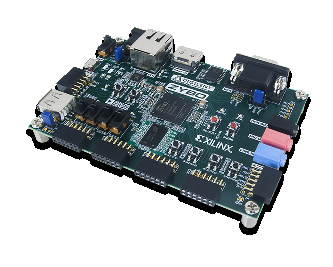
\includegraphics[width=4cm]{./graphics/zybo}
    \end{center}
	\end{block}
\end{frame}


%%%%%%%%%%%%%%%%%% ATTACK SECTION %%%%%%%%%%%%%%%%%%%%

\section{Attack}
\subsection{Statistical tool}
\begin{frame}[fragile]
	\frametitle{Finding correlations}
	\begin{block}{PCC: our game changer}
		In order to find the linear contribution of each sample in the overall time, we have used the \textit{Pearson Correlation Coefficient} as an estimator. It has proved to be really effective for our needs, working on the realizations of a random variable.
	\end{block}
	\begin{center}
		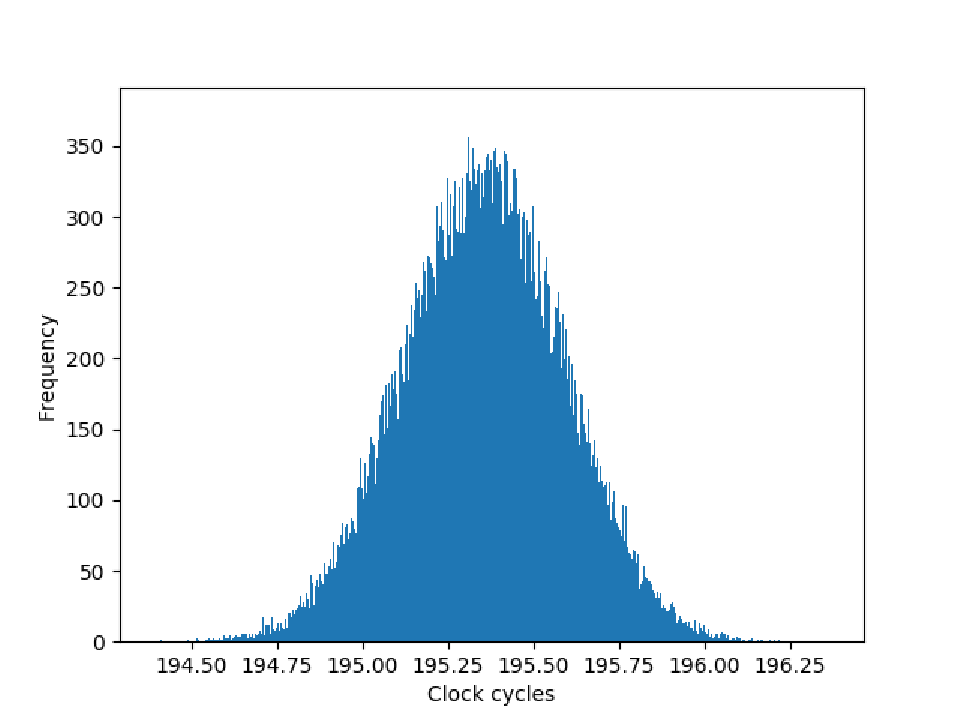
\includegraphics[width=6cm]{./graphics/rand_distr}
	\end{center}
\end{frame}

\subsection{Algorithm}

\begin{frame}[fragile]
    \frametitle{Algorithm}
    \begin{block}{Development}
        \begin{itemize}
            \pause \item Started in Python to allow better flexibility and library support (infinite precion, \texttt{scipy.stats})
            \pause \item At first, attacking conditional Montgomery Mult., 1 bit at-a-time, using fixed threshold
            \pause \item Move on to attack both MM to improve statistical relevance of 0 guesses
            \pause \item Get rid of fixed threshold by: using multi bit analysis and taking max between the accumulated PCCs on a common path
        \end{itemize}
    \end{block}

\end{frame}


\begin{frame}[fragile]
    \frametitle{Algorithm}
    \begin{block}{Final implementation}
        \begin{itemize}
            \pause \item Attack at the same time the two Montgomery moltiplications present in an RSA iteration
            \pause \item Timing estimate: dummy Montgomery moltiplication which evaluates the number of taken branches
            \pause \item Multi bit guessing
            \pause \item Error-detection capabilities
        \end{itemize}
    \end{block}
    \hfill 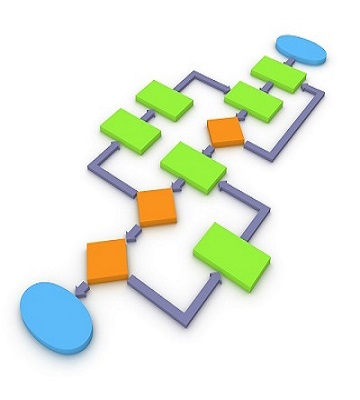
\includegraphics[width=2cm]{./graphics/algorithm}
\end{frame}

\begin{frame}[fragile]
    \frametitle{Algorithm}
    \begin{block}{Optimizations}
        \begin{itemize}
            \pause \item Completely rewritten in C with +10x speedup over Python
            \pause \item Fully customizable number of bits considered and guessed in one attack iteration
            \pause \item Tweakable filtering of input data with \texttt{\#define} parameters for noisy samples
        \end{itemize}
    \end{block}
    \hfill 
\includegraphics[width=2cm]{./graphics/tweak}
\end{frame}

\begin{frame}[fragile]
    \frametitle{Algorithm}
    \begin{block}{To have an idea...}
        The C implementations, running on a machine with 2.4Ghz Intel i5:
        \begin{itemize}
            \pause \item cracks 128-bit RSA in 3m40sec
            \pause \item using 10k plaintexts sampled on Zybo board
            \pause \item considering 2 bits and guessing 1 per iteration of the attack
        \end{itemize}
    \end{block}
    \hfill 
\includegraphics[width=3cm]{./graphics/hacker}
\end{frame}

\subsection{Extremely powerful}
\begin{frame}{Just a simplification}
	\begin{block}{Works on computer also}
		Even if we mainly worked on the \textit{Zybo} board, we can claim that:
		\begin{itemize}
			\pause \item our attack works also when mounted for other devices, including different architectures (Intel x86, ..)
			\pause \item with an  OS, more tuples (cipher, timing) are needed
			\pause \item the attack is still feasible
		\end{itemize}
    We have completely tested what is mentioned above.
    \begin{center}
      
\includegraphics[width=4cm]{./graphics/pc}
    \end{center}
	\end{block}
\end{frame}

\begin{frame}{Bigger keys}
  \begin{center}
    
\includegraphics[width=4cm]{./graphics/key}
  \end{center}
  \begin{block}{RSA on 512/1024/2048/4096}
		The algorithm is capable of handling larger keys on 512, 1024, 2048 and 4096 bits.
    However, the processing time is longer, and a more complex backtrack might be necessary in some cases.
	\end{block}
\end{frame}

\section{Counter}

\begin{frame}[fragile]
\frametitle{Titlepage settings}
\begin{itemize}
\pause \item by changing settings in \begin{verbatim} header_footer.sty \end{verbatim} you can choose whether and where you want a second logo to be positioned on the titlepage:
\begin{itemize}
\pause \item small logo can be placed on the bottom right
\pause \item big logo can be placed on the top right
\end{itemize}
\pause \item spaces and graphics dimensions will have to be adjusted depending on your logo
\end{itemize}
\end{frame}

\begin{frame}[fragile]
\frametitle{Outline}
\begin{itemize}
\pause \item divide the presentation, using the command {\tt section}
(as it is usually done in \LaTeX)
\pause \item other divisions, just as chapter or part are not supported
\pause \item the sections are are listed on the top of each slide, the section the
recent slide belongs to is highlighted
\pause \item you can automatically receive an outline out of this section by the command
\begin{verbatim}
\tableofcontents
\end{verbatim}
\end{itemize}
\end{frame}


\section{Possibilities}

\begin{frame}
\frametitle{Itemize}
\begin{itemize}
\pause \item black circle is the default; other possibilities are:
\begin{itemize}
\pause \item ball
\begin{itemize}
\pause \item triangle
\end{itemize}
\end{itemize}
\pause \item the color of the items can also be changed
\pause \item all this settings have to be done in the preamble of the {\tt presentation.tex} file
\end{itemize}
\end{frame}

\begin{frame}
\frametitle{Overlays}
\begin{itemize}
\onslide+<2-> {\pause \item its possible to build slides succesively}
\onslide+<3-> {\pause \item to do so use the command {\tt onslide} }
\onslide+<4-> {\pause \item other useful commands are {\tt uncover} and {\tt only} }
\onslide+<5-> {\pause \item this works also very nice to ''develop'' formulas: }
\[
\onslide+<6-> {f (x \mid \mu, \sigma^2) ~=~ }
\onslide+<7-> { \frac 1 {\sigma\sqrt{2\pi}} }
\onslide+<8-> { \cdot \exp\left\{ }
\onslide+<9-> { -\frac {(x-\mu)^2} {2\sigma^2} }
\onslide+<8-> { \right\} }
\]

\end{itemize}
\end{frame}


\section{Graphics}

\begin{frame}[fragile]
\frametitle{Pimp up your presentation}
\begin{itemize}
\pause \item an easy way to include pictures is by using
\begin{verbatim}
\includegraphics[width=...,height=...]{file}
\end{verbatim}
\pause \item in connection with {\tt pdflatex} this supports a wider range of graphic formats, including GIF, PNG, JPG \\[0.3cm]
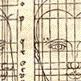
\includegraphics[width=2cm,height=2cm]{./graphics/FF4.jpg}
\end{itemize}
\end{frame}

\section{Useful Hints}

\begin{frame}[fragile]
\frametitle{Useful hints}
\begin{itemize}
\pause \item if you use a verbatim environment on a slide, declare that slide {\tt fragile}:
\begin{verbatim}
\begin{frame}[fragile]
\end{verbatim}
\pause \item bibliography actually works as usual, just keep in mind that not all bibliography styles are supported by the {\it beamer}
      package, maybe you have to include some other packages to get your preferred style working
\end{itemize}
\end{frame}

\nocite{*}



%%%%%%%%%%%%%%%%%%%%%%%% COUNTERMEASURES %%%%%%%%%%%%%%%%%%%

\section{Countermeasures}
\begin{frame}{Possible solution}
    \begin{block}{Blinding}
		The proposed countermeasure is the one given in \cite{kocher1996timing}.
		It consists in blinding the message before the encryption using a couple of values $v_f, v_i$ chosen in such a way that:
		\begin{equation*}
			v_i^e \cdot v_f mod\: N = 1
		\end{equation*}
        This contermeasure, in all our tests, has proven to be really effective. Ciphers are completely masked, no correlation can be identified.
    \end{block}
\end{frame}

\begin{frame}{Possible solution}
    \begin{block}{Blinding}

    \end{block}
\end{frame}

\begin{frame}{Future expectations}
  \begin{block}{What more}
    \begin{itemize}
      \pause \item porting the attack in C++ to keep class structure and speedup w.r. to Python
      \pause \item find an optimal filter and explain the strange behavior of the implemented filter
      \pause \item try to parallelize the estimation for all the messages, as every message is data-independent from each other
    \end{itemize}
  \end{block}
\end{frame}

\begin{frame}{Our team}
  \noindent
  \begin{minipage}[l][\dimexpr.45\textheight-2\fboxsep-2\fboxrule\relax][t]{\dimexpr .495\textwidth-2\fboxsep-2\fboxrule\relax}
      \begin{center}
        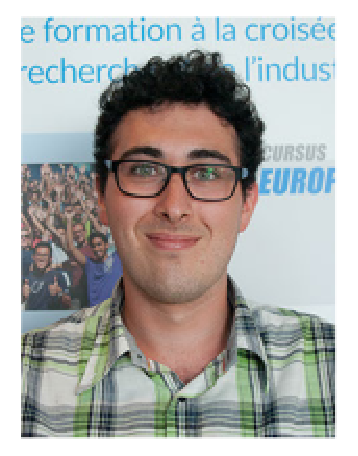
\includegraphics[height=2.7cm]{./graphics/anselmo}\\
        ANSELMO, Alberto
      \end{center}
  \end{minipage}%
  \hfill
  \begin{minipage}[r][\dimexpr 0.45\textheight-2\fboxsep-2\fboxrule\relax][t]{\dimexpr .495\textwidth-2\fboxsep-2\fboxrule\relax}%
      \begin{center}
        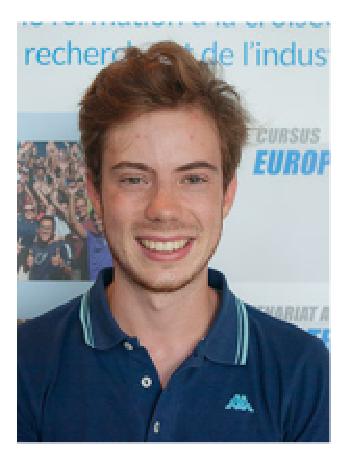
\includegraphics[height=2.7cm]{./graphics/chiaberto}\\
        CHIABERTO, Simone
      \end{center}
  \end{minipage}%
  \vfill
  \noindent
  \begin{minipage}[l][\dimexpr 0.45\textheight-2\fboxsep-2\fboxrule\relax][t]{\dimexpr .495\textwidth-2\fboxsep-2\fboxrule\relax}%
      \begin{center}
        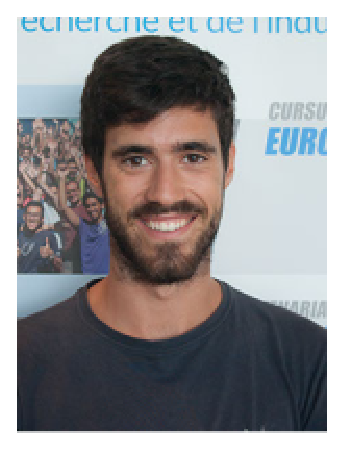
\includegraphics[height=2.7cm]{./graphics/chiatante}\\
        CHIATANTE, Fausto
      \end{center}
  \end{minipage}%
  \hfill
  \begin{minipage}[r][\dimexpr 0.45\textheight-2\fboxsep-2\fboxrule\relax][t]{\dimexpr .495\textwidth-2\fboxsep-2\fboxrule\relax}%
    \begin{center}
      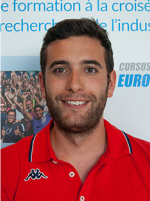
\includegraphics[height=2.7cm]{./graphics/roggero}\\
      ROGGERO, Giulio
    \end{center}
  \end{minipage}%
\end{frame}

\begin{frame}[allowframebreaks]
	\frametitle{References}
%\Large{References} \\[0.5cm]
	\footnotesize
	\bibliographystyle{apalike}
	\bibliography{./bibliography/LaTeX}
\end{frame}

\end{document}
